\scanpage{107}
\figure{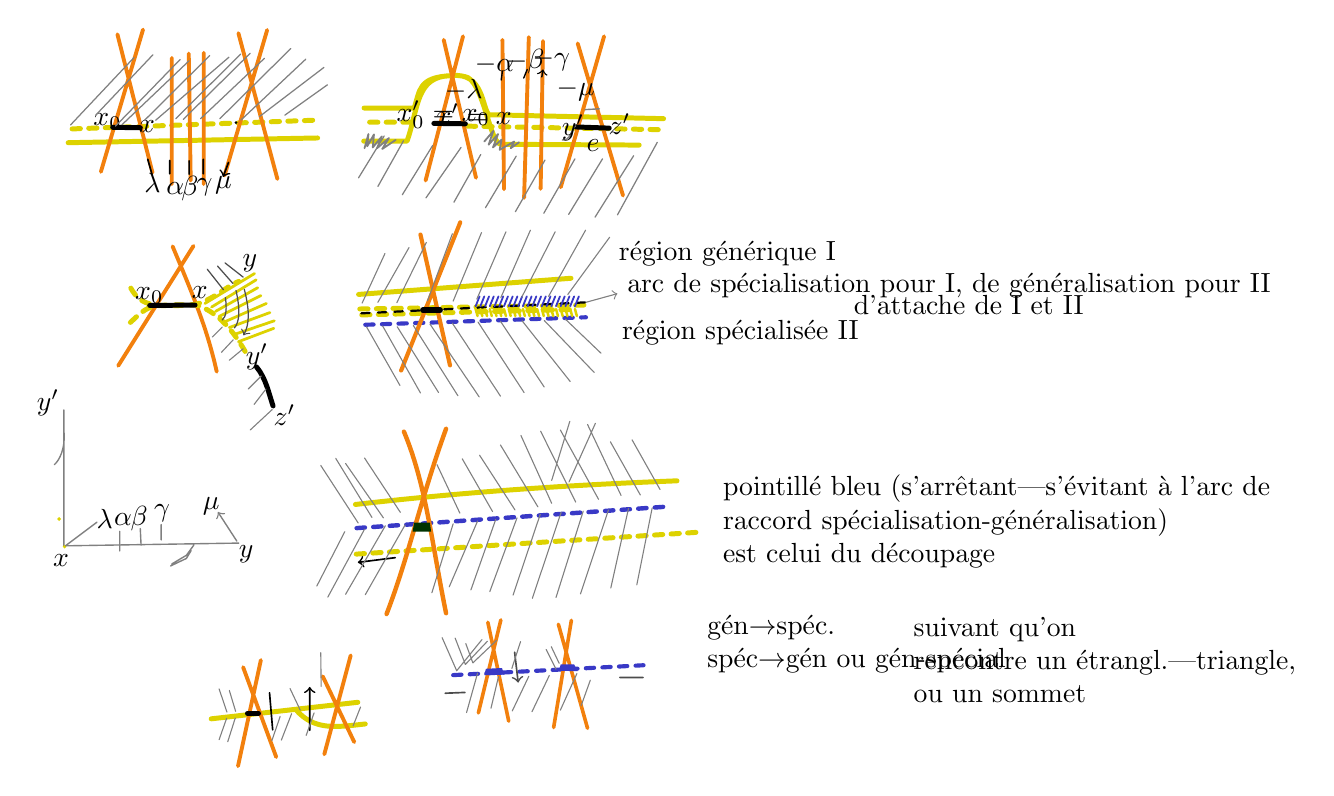
\begin{tikzpicture}[x=.005cm,y=-.005cm,line cap=round,line join=round]
\draw[yellow!70!olive,line width=1.8pt] (226,524)--(859,512);
\draw[yellow!70!olive,line width=1.8pt,dashed] (236,489)--(849,467);
\draw[orange!80!brown,line width=1.4pt] (351,249)--(440,600) (416,237)--(309,598) (658,246)--(757,616) (731,238)--(623,607) (489,309)--(489,629) (532,298)--(537,620) (570,296)--(570,629);
\draw[black,line width=1.8pt] (339,485)--(409,486);
\draw[black,->,line width=.6pt] (428,566)--(439,605) (484,569)--(484,603) (533,570)--(533,604) (569,566)--(569,603) (633,574)--(619,611);
\fill[black] (652,473) circle (4);
\node at (326,471) {$x_0$};\node at (426,482) {$\unsure{x}$};\node at (440,627) {$\lambda$};\node at (498,641) {$\alpha$};\node at (535,641) {$\beta$};\node at (572,638) {$\gamma$};\node at (620,633) {$\mu$};
\draw[gray,line width=.45pt] (232,479)--(393,308) (296,454)--(441,301) (346,482)--(510,313) (363,478)--(533,316) (420,467)--(585,303) (448,467)--(634,307) (499,463)--(664,299) (518,465)--(688,297) (562,463)--(724,310) (611,463)--(791,285) (665,466)--(829,312) (711,458)--(875,333) (776,454)--(884,377);
\draw[yellow!70!olive,line width=1.8pt] (977,436)--(1104,436)..controls(1119,393)and(1113,357)..(1199,354)..controls(1281,344)and(1276,437)..(1294,453)--(1737,463) (976,520)--(1086,520)..controls(1116,434)and(1108,354)..(1199,354) (1232,356)..controls(1280,362)and(1295,529)..(1325,528)--(1675,530);
\draw[yellow!70!olive,line width=1.8pt,dashed] (991,472)--(1117,472) (1239,482)--(1733,491);
\draw[orange!80!brown,line width=1.4pt] (1179,263)--(1261,613) (1228,254)--(1133,620) (1519,272)--(1634,658) (1586,254)--(1476,637) (1328,263)--(1332,642) (1395,256)--(1383,664) (1431,266)--(1425,641);
\draw[black,line width=1.8pt] (1154,475)--(1234,476) (1514,484)--(1599,487);
\draw[gray,line width=.5pt] (1538,440)--(1574,438) (1480,517)..controls(1501,521)and(1503,487)..(1514,481);
\draw[black,->,line width=.5pt] (1325,365)--(1328,342) (1382,360)--(1391,338) (1428,357)--(1431,338);
\node at (1230,390) {$-\lambda$};\node at (1308,326) {$-\alpha$};\node at (1386,318) {$-\beta$};\node at (1452,315) {$-\gamma$};\node at (1514,391) {$-\mu$};
\node at (1178,453) {$\unsure{x'_0=x_0}$};\node at (1255,451) {$\unsure{x'=x}$};\node at (1507,485) {$y^{\prime}$};\node at (1625,476) {$z^{\prime}$};\node at (1558,532) {$\unsure{e}$};
\draw[gray,line width=.45pt] (963,613)--(1028,507) (1012,635)--(1077,519) (1074,656)--(1151,531) (1134,664)--(1223,536) (1205,675)--(1273,554) (1285,689)--(1363,558) (1361,699)--(1436,568) (1433,703)--(1512,565) (1496,706)--(1582,565) (1563,713)--(1661,557) (1620,707)--(1721,523);
\draw[gray,line width=.65pt] (978,538)--(988,502)--(985,533)--(1002,503)--(999,536)--(1022,508)--(1010,538)--(1040,512)--(1023,540)--(1057,517) (1282,521)--(1305,494)--(1293,529)--(1317,502)--(1304,536)--(1326,516)--(1321,542)--(1358,521)--(1349,538)--(1370,523);
\draw[orange!80!brown,line width=1.4pt] (491,787)..controls(552,932)and(580,1003)..(603,1105) (544,786)--(353,1090);
\draw[yellow!70!olive,line width=1.8pt,dashed] (385,893)..controls(412,941)and(446,941)..(549,935)..controls(608,953)and(649,1006)..(681,1064) (384,980)..controls(436,931)and(431,937)..(548,935)..controls(603,918)and(630,886)..(659,876);
\draw[black,line width=1.8pt] (433,937)--(548,936) (704,1093)..controls(728,1122)and(735,1160)..(746,1192);
\node at (432,911) {$x_0$};\node at (560,904) {$x$};\node at (687,831) {$y$};\node at (705,1067) {$y^{\prime}$};\node at (775,1215) {$z^{\prime}$};
\draw[yellow!70!olive,line width=1pt] (573,932)--(699,856) (590,941)--(703,872) (600,952)--(707,892) (609,965)--(715,912) (622,979)--(729,932) (635,993)--(738,955) (646,1011)--(749,976) (658,1029)--(748,995);
\draw[black!70,->,line width=.45pt] (579,845)--(620,897) (605,837)--(644,881) (624,829)--(670,865) (625,917)..controls(629,945)and(627,966)..(617,974) (652,899)..controls(663,949)and(661,978)..(648,994) (673,896)..controls(687,951)and(686,984)..(671,1013);
\draw[gray,line width=.4pt] (617,992)--(592,1017) (645,1024)--(615,1056) (670,1047)--(635,1076) (716,1116)--(683,1149) (728,1149)--(698,1188) (744,1201)--(688,1253);
\draw[yellow!70!olive,line width=1.8pt] (963,909)--(1502,868);
\draw[yellow!70!olive,line width=1.8pt,dashed] (966,946)--(1535,936) (971,961)--(1509,947);
\draw[blue!55!gray,line width=1.5pt,dashed] (980,986)--(1540,967);
\draw[orange!80!brown,line width=1.5pt] (1120,757)--(1195,1089) (1221,726)--(1071,1102);
\draw[black,line width=2pt] (1126,949)--(1170,949);
\draw[black,dashed,line width=.8pt] (970,957)--(1541,929);
\draw[gray,->,line width=.4pt] (1540,929)--(1620,907);
\foreach \x in {1260,1272,1284,1296,1308,1320,1332,1344,1356,1368,1380,1392,1404,1416,1428,1440,1452,1464,1476,1488,1500,1512}{\draw[blue!55!gray,line width=.65pt] (\x,939)--++(10,-25);\draw[yellow!70!olive,line width=.9pt] (\x,946)--++(5,18);}
\draw[gray,line width=.4pt] (972,931)--(1030,805) (1012,929)--(1091,790) (1060,930)--(1135,777) (1138,925)--(1201,755) (1203,926)--(1275,752) (1263,921)--(1337,750) (1324,917)--(1399,746) (1377,916)--(1462,750) (1445,914)--(1539,746) (1494,909)--(1600,764);
\draw[gray,line width=.4pt] (983,991)--(1068,1140) (1024,989)--(1120,1159) (1061,991)--(1166,1158) (1102,988)--(1215,1166) (1144,984)--(1269,1169) (1201,982)--(1323,1167) (1266,979)--(1383,1158) (1323,977)--(1434,1144) (1378,976)--(1500,1130) (1434,975)--(1561,1107) (1488,972)--(1578,1058);
\node[anchor=west] at (1599,806) {région générique $\mathrm{I}$};
\node[anchor=west] at (1620,886) {arc de spécialisation pour $\mathrm{I}$, de généralisation pour $\mathrm{II}$};
\node[anchor=west] at (2195,935) {d'attache de $\mathrm{I}$ et $\mathrm{II}$};
\node[anchor=west] at (1607,1007) {région spécialisée $\mathrm{II}$};
\draw[gray,line width=.5pt] (215,1202)--(215,1547)--(659,1540) (216,1261)..controls(218,1299)and(205,1329)..(191,1341) (545,1545)--(526,1571)--(489,1593) (538,1559)--(526,1579)--(486,1598);
\fill[yellow!70!olive] (203,1479) circle (5);\fill[yellow!70!olive] (217,1549) circle (5);
\draw[gray,->,line width=.5pt] (219,1547)--(299,1487) (357,1560)--(357,1510) (411,1545)--(409,1503) (462,1532)--(462,1493) (654,1535)--(606,1461);
\node at (175,1184) {$y^{\prime}$};\node at (208,1584) {$x$};\node at (678,1569) {$y$};\node at (319,1478) {$\lambda$};\node at (365,1480) {$\alpha$};\node at (406,1477) {$\beta$};\node at (464,1465) {$\gamma$};\node at (589,1446) {$\mu$};
\draw[yellow!70!olive,line width=1.8pt] (955,1442)..controls(1210,1413)and(1460,1394)..(1771,1382);
\draw[blue!55!gray,line width=1.6pt,dashed] (958,1502)--(1739,1448);
\draw[yellow!70!olive,line width=1.8pt,dashed] (957,1568)--(1833,1512);
\draw[orange!80!brown,line width=1.6pt] (1078,1257)..controls(1134,1391)and(1148,1536)..(1185,1718) (1185,1250)..controls(1119,1432)and(1091,1572)..(1034,1720);
\fill[green!20!black] (1104,1488)--(1144,1488)--(1147,1511)--(1100,1511)--cycle;
\draw[black,->,line width=.6pt] (1056,1577)--(961,1589);
\draw[gray,line width=.4pt] (867,1343)--(962,1489) (905,1325)--(997,1475) (930,1338)--(1026,1476) (978,1324)--(1069,1462) (1162,1341)--(1220,1464) (1226,1326)--(1303,1460) (1270,1317)--(1360,1456) (1323,1291)--(1418,1448) (1375,1267)--(1453,1439) (1425,1256)--(1514,1436) (1475,1253)--(1572,1429) (1544,1239)--(1629,1419) (1602,1283)--(1678,1418) (1657,1278)--(1728,1404) (1453,1381)--(1499,1231) (1497,1385)--(1564,1236);
\draw[gray,line width=.4pt] (928,1511)--(857,1649) (978,1505)--(885,1677) (1031,1496)--(930,1670) (1081,1494)--(980,1671) (1203,1491)--(1149,1666) (1265,1484)--(1193,1651) (1311,1480)--(1248,1659) (1365,1476)--(1296,1663) (1424,1467)--(1355,1672) (1477,1462)--(1404,1680) (1533,1459)--(1464,1678) (1597,1456)--(1526,1669) (1648,1452)--(1603,1654) (1708,1451)--(1669,1646);
\node[anchor=west,align=left] at (1863,1485) {pointillé bleu (\unsure{s'arrêtant|s'évitant} à l'arc de\\raccord spécialisation-généralisation)\\est celui du découpage};
\draw[yellow!70!olive,line width=1.8pt] (589,1986)--(961,1944) (803,1962)..controls(851,2017)and(906,2007)..(980,1999);
\draw[orange!80!brown,line width=1.4pt] (670,1855)--(754,2083) (715,1837)--(657,2106) (872,1878)--(952,2045) (943,1825)--(876,2076);
\draw[black,line width=1.8pt] (681,1972)--(709,1972);
\draw[black,->,line width=.6pt] (737,1920)--(745,2014) (839,2015)--(839,1905);
\draw[gray,line width=.4pt] (609,1910)--(629,1969) (635,1914)--(651,1967) (789,1909)--(815,1964) (867,1818)--(868,1904) (628,1985)--(609,2039) (650,1984)--(631,2044) (764,1980)--(743,2041) (793,1973)--(767,2040) (850,1971)--(830,2028) (968,1956)--(949,2004);
\draw[blue!55!gray,line width=1.5pt,dashed] (1203,1875)--(1686,1850);
\draw[orange!80!brown,line width=1.3pt] (1291,1741)--(1344,1992) (1324,1735)--(1267,1971) (1470,1746)--(1544,2010) (1503,1736)--(1458,2008);
\fill[blue!55!gray] (1286,1859)--(1327,1857)--(1332,1874)--(1282,1875)--cycle (1476,1848)--(1510,1848)--(1519,1865)--(1471,1864)--cycle;
\draw[black!70,->,line width=.6pt] (1233,1919)--(1183,1921) (1626,1881)--(1685,1881) (1359,1817)--(1368,1894);
\draw[gray,line width=.4pt] (1175,1780)--(1212,1864)--(1276,1785) (1208,1781)--(1234,1848)--(1290,1789) (1235,1795)--(1253,1844)--(1313,1787) (1265,1870)--(1237,1970) (1318,1879)--(1299,1959) (1395,1878)--(1353,1966) (1447,1876)--(1403,1968) (1517,1871)--(1475,1964) (1551,1888)--(1528,1952) (1439,1810)--(1464,1860) (1452,1803)--(1472,1845) (1374,1790)--(1352,1858);
\node[anchor=west,align=left] at (1823,1797) {gén$\to$spéc.\\spéc$\to$gén ou \unsure{gén-spécial}};
\node[anchor=west,align=left] at (2347,1837) {suivant qu'on\\rencontre un \unsure{étrangl.|triangle},\\ou un sommet};
\end{tikzpicture}}
\margin{106}
